\chapter{Estado del arte} % Main chapter title

\label{EstadoDelArte} % For referencing the chapter elsewhere, use \ref{Chapter1} 

\lhead{Capítulo \ref{EstadoDelArte}. \emph{Estado del arte}} 

En éste capítulo se va a hacer un recuento de los diferentes enfoques y técnicas que se han utilizado para atacar el problema de la simulación y control de los músculos del cuerpo humano. Basándose en su metodología fundamental, se clasificaron los diferentes enfoques en las siguientes categorías: deformación muscular, control y simulación, y simulación basada en fibras.

\section{Deformación muscular}

Los músculos proveen las funciones fisiológicas que generan el movimiento del cuerpo y le dan forma, haciendo que sean un componente clave en la animación y modelado de figuras humanas. Una deformación realista de los músculos es necesaria para tener personajes humanoides animados de alta calidad. Hay muchos trabajos que desarrollan modelos matemáticos, físicos, y computacionales para la simulación de músculos (desde un músculo hasta cuerpos completos) con el propósito de aumentar su realismo y exactitud en una amplia gama de aplicaciones: video juegos y películas, realidad virtual y aumentada, telepresencia, medicina, biomecánica, entre otras. 

Dependiendo de distintos requerimientos de desempeño y visualización, cada uno de los trabajos toma un distinto enfoque con respecto al modelado de sus simulaciones. Por ejemplo, realismo visual es deseable en producciones de cine, o videojuegos, por lo que hay un enfoque mayor en la graficación y visualización de los músculos; mientras que exactitud anatómica o biomecánica es preferible en aplicaciones médicas, por lo que enfocarse en su correcto funcionamiento tiene prioridad. 

A pesar de la cantidad de trabajo, la complejidad del cuerpo humano y sus músculos, hacen de su modelado sea todo un reto. En el presente capítulo se mencionan distintos trabajos que han atacado el reto de el modelado y el control de los músculos esqueléticos del cuerpo. En ésta parte se hace énfasis en distintos trabajos que han atacado el problema de la deformación muscular con distintos enfoques: enfoques geométricos, enfoques basados en física, y enfoques basados en datos.

\subsection{Enfoques geométricos}

Los enfoques geométricos se emplearon en las primeras simulaciones realizadas debido a que son prácticos y eficientes. La mayoría de los trabajos realizados se enfocan en modelar los efectos de la animación de la contracción muscular, como el abultamiento o la hinchazón, que pueden ser factores fundamentales para la deformación de la piel, o para animaciones faciales. Éstos han sido exitosos en el modelado de músculos simples (por ejemplo, los fusiformes) pero puede que no haya una extensión directa a los músculos complejos \citep{Scheepers:1997, wilhelms1997anatomically}. Además, como la deformación de los músculos se determina por el arreglo de los huesos, estas técnicas tienen problemas para lograr un nivel alto de realismo desde perspectivas fisiológicas o biomecánicas. Por esto, para manejar mejor esos problemas, los músculos se construyen en varias capas, o se les aplican enfoques físicos.

Chadwick et al. \citep{Chadwick:1989} utilizó Deformaciones de Forma Libre (Free Form Deformations, FFDs) para representar la deformación muscular. Un esqueleto articulado transforma un enrejado de FFDs, que a su vez representa el cambio de forma de un músculo, como se pude ver en la \fref{fig:FFDLatice}. Aunque las FFDs proveen una forma simple de control, no permiten una manipulación directa, y no permiten producir formas más complejas. Moccozet et al. \cite{moccozet1997dirichlet} aborda dicha limitación al introducir Deformaciones de Forma Libre de Dirichlet (Dirichlet Free Form Deformations, DFFDs) las cuales están basadas en una técnica de interpolación de datos dispersos. Ellos remueven el requerimiento de puntos de control espaciados regularmente al reemplazar coordenadas rectangulares locales por coordenadas vecinas naturales (es decir, coordenadas Sibson). Dado un punto, sus vecinos naturales son recolectados basados en diagramas de Delaunay y Dirichlet/Voronoi, y su desplazamiento es calculado utilizando interpolación. Ellos usan un modelo de deformación de multi-capas para generar animaciones de manos donde la capa muscular es modelada por un conjunto de puntos de control de DFFD que corresponde a una topografía simplificada de una mano.

\begin{figure}
	\centering
		\includegraphics[scale=0.5]{FDDLatice.png}
		\caption[Ejemplo de la deformación de una superficie de FFD para un brazo.]{Ejemplo de la deformación de una superficie de FFD para un brazo. En la parte superior se puede ver como el movimiento del brazo modifica la superficie de FFD. La parte inferior muestra el efecto del movimiento con una piel geométrica basada en superficies paramétricas. Adaptado de \citep{Chadwick:1989}.}
		\label{fig:FFDLatice}
\end{figure}

Komatsu \cite{komatsu1988human} utilizó superficies de Bezier para modelar la deformación del cuerpo. Las superficies se parchan cilíndricamente alrededor de un esqueleto, y se controlan en conjunto para transformar el cuerpo. Wilhelms \cite{wilhelms1997animals} y Scheepers et al. \cite{Scheepers:1997} utilizaron elipsoides paramétricos como la primitiva básica para modelar los vientres musculares de los músculos esqueletales del cuerpo humano. Ellos ajustan tres ejes principales para representar el abultamiento de los músculos, mientras que el volúmen se preserva utilizando relaciones predefinidas entre dichos ejes. Aunque un elipsoide es suficiente para modelar formas simples, como un músculo fusiforme, no se puede adaptar fácilmente para modelar formas más complejas. El trabajo de Scheepers et al. se distingue ya que extiende el modelo básico de elipsoides para representar músculos con múltiples vientres (por ejemplo, el pectoralis) en donde n pares de puntos de origen e inserción se especifican, y n elipsoides se alinean lateralmente a lo largo de cada par. Ése modelo se usa para representar músculos más complejos que son doblados o envueltos alrededor de una estructura (por ejemplo, el brachioradialis en el antebrazo). El camino directo entre los puntos de origen e inserción se reemplaza por una curva de Bezier que representa la dirección de la fuerza del músculo, y por elipses de tamaños variados a lo largo de dicha curva para definir el volumen y la forma del músculo. Wilhelms and Gelder \cite{wilhelms1997anatomically} presentan un trabajo donde se utilizan cilindros con cortes transversales para representar los músculos. Cada corte transversal es modelado utilizando curvas B-Spline y su radio es controlado para expresar los cambios volumétricos en el músculo. Los cilindros también se pueden doblar para modelar músculos que se doblan en las uniones del cuerpo. Además, la longitud, el ancho, y el grueso del músculo se escalan para mantener un volumen constante. Esta forma de modelado se puede ver en la\fref{fig:cilinderDeformation}.

\begin{figure}
	\centering
		\includegraphics[scale=0.8]{cilinderDeformation.png}
		\caption[Ejemplo de la deformación de un cilindro con cortes transversales.]{La forma del músculo se define por el control de los cortes transversales del cilindro. La parte superior muestra el músculo con una piel, mientras que la parte inferior muestra el cilindro deformado. Adaptado de \citep{wilhelms1997anatomically}.}
		\label{fig:cilinderDeformation}
\end{figure}

Ramos y Larboulette \citep{ramos2013muscle} presentan un método para deformar la piel de personajes utilizando los músculos subyacentes. Para simular los músculos, utilizan curvas paramétricas para generar las distintas formas de los músculos. La forma general de su modelo de músculos es un cilindro generalizado definido por el barrido de una curva de grosor $C_T(t)$ a lo largo de una curva de barrido $C_S(t)$. $C_S(t)$ es una curva de Bezier tridimensional que representa el perfil del músculo. Esa curva se define por dos puntos: el origen \textbf{O} y la inserción \textbf{I} del músculo. $C_S(t)$ es una función que representa el grueso del músculo como una función de $t$. De esta manera, cada sección del músculo en $t$ se define por una elipse que esta a lo largo de $C_S(t)$ cuyo grosor esta dado por $C_T(t)$. Cada una de las curvas de Bezier $C_S(t)$ y $C_T(t)$ están compuestas por dos curvas de Bezier llamadas \textit{el segmento de origen} y \textit{el segmento de inserción}. Cada una de esas curvas tiene cuatro puntos de control $p_j, j \in [0,3]$. En la \fref{fig:cylinderCurves} se puede ver una representación de las curvas y su efecto en el modelado de un músculo.

\begin{figure}
	\centering
		\includegraphics[scale=0.8]{cylinderCurves.png}
		\caption[Deformación de un cilindro con curvas de Bezier.]{En la parte superior se ve la curva $C_T(t)$; en el centro la curva $C_S(t)$; en la parte inferior se ve la sección longitudinal resultante de barrer $C_T(t)$ a lo largo de $C_S(t)$, representando $C_S(t)$ como una línea punteada. Adaptado de \citep{ramos2013muscle}.}
		\label{fig:cylinderCurves}
\end{figure}

Una parte importante de éste modelo de músculos es que se considera la tensión generada por contracciones isométricas e isotónicas. En el caso de contracciones isométricas, los huesos no se mueven y la longitud del músculo no cambia. Sin embargo, su forma sí se modifica. Cuando la tensión aumenta, el músculo se abulta en una dirección mientras se estrecha perpendicularmente. En una contracción isotónica, los huesos se mueven pero la tensión en el músculo permanece constante. El cambio en la forma ocurre solamente por el acortamiento o la elongación del músculo. Si se acorta, el vientre muscular se abulta; decrece en el caso opuesto. Desventajas de éste modelo son que no se considera una interacción entre músculos o entre músculos y huesos, y solamente se modelan los músculos más superficiales. 

Otro enfoque geométrico utilizado es el de las superficies implícitas. Una superficie implícita generada por un juego de esqueletos, $ s_i (i=1,2,\dots,n)$, con una función de campo asociada, $ f_i$, esta definida en el isovalor $c$ por:

\begin{equation}
	\{P\in\mathbb{R}^3 | f(P) = c \}  \text{  donde  }  f(P) = \sum_{i=1}^{n} f_i(P)
\end{equation}

El esqueleto, $s_i$, puede ser cualquier primitiva geométrica como un punto, una curva, o una superficie paramétrica. La función de campo, $f_i$, es generalmente una función decreciente de distancia desde un punto dado, $P$, al esqueleto asociado. Dependiendo del tipo de función de campo, se han desarrollado varias superficies implícitas: blobs, metaballs, objetos suaves, y superficies de convolución \citep{blinn1982generalization, wyvill1988field, bloomenthal1991convolution}.

Bloomenthal et al. \citep{bloomenthal1991convolution} utilizó superficies de convolución para modelar una mano y brazo humanos, al aproximar huesos, músculos, tendones, y venas, al esqueleto subyacente. Thalmann et al. \citep{thalmann1996fast} presentó un modelo de un humano basado en múltiples capas, donde las primitivas del cuerpo (es decir, músculos, extremidades, tejidos, etc) eran construidos a partir de un esqueleto de lineas que era cubierto con superficies elipsoidales de metaballs (ver \fref{fig:layeredHumanConstruction}). Aunque las superficies implícitas son suaves y continuas  al momento de modelar objetos, se pueden producir efectos no deseados de mezclado al momento de modelar deformaciones en uniones del cuerpo. 

\begin{figure}
	\centering
		\includegraphics[scale=0.8]{layeredHumanConstruction.png}
		\caption[Construcción por capas de un cuerpo humano.]{Construcción por capas de un cuerpo humano. Adaptado de \citep{thalmann1996fast}.}
		\label{fig:layeredHumanConstruction}
\end{figure}

\subsection{Enfoques basados en física}

Aunque los modelos geométricos han probado ser suficientes para algunas aplicaciones gráficas que demandan una calidad visual aceptable, su simplicidad y la necesidad de intervención humana para configurar los modelos, usualmente hace que sea difícil extenderlos para representar escenas complejas que involucren dinámica. Además, no tienen la precisión física o mecánica que es requerida para generar modelos, animaciones, y simulaciones más realistas. Por esto, muchos investigadores han trabajado en modelos donde problemas complicados como la dinámica de las propiedades de músculos y tejidos se resuelven con física. Para modelar músculos basados en física, se tienen que considerar los siguientes problemas: 1) determinar las fuerzas contráctiles de los músculos, y 2) representar la geometría cambiante de los músculos durante una contracción. Para resolver estos problemas, se han generado varios modelos de músculos basados en una variedad de métodos computacionales, como sistemas masa-resorte, Método de Elemento Finito (FEM, Finite Element Method), Método de Volumen Finito (FVM, Finite Volume Method), y más recientemente, simulaciones de sólidos Eulerianos.

\subsubsection{Sistemas de masa-resorte}

En el caso de los sistemas de masa-resorte, un objeto es modelado como una colección de puntos de masa vinculados entre si mediante resortes sin masa. Una fuerza elástica que actúa sobre una masa $i$ conectada por un resorte a la masa $j$ está dada por:

\begin{equation}
	f_ij = k(|x_ij| -l_ij)\frac{x_ij}{|x_ij|}
\end{equation}

donde $x_ij = x_j - x_i$, y $x_i$, $x_j$ son posiciones de puntos de masas $i$ y $j$, respectivamente, $l_ij$ es la longitud de descanso entre ellos y $k$ es la rigidez del resorte. Este modelo lineal de resorte se puede generalizar al incorporar varios tipos de fuerzas de resorte, como fuerzas angulares, o de doblez. 

Chadwick et al. \citep{Chadwick:1989}, vinculó los puntos de control de FFD a puntos de masa en un sistema de masa-resorte, permitiendo que el sistema dinámico influyera en las deformaciones basadas en geometría. Al aumentar el modelo de músculos basado en FFD con el sistema de masa-resorte, fueron capaces de representar propiedades visco-elásticas que simulaciones basadas en esqueletos articulados normalmente no tienen. Lee et al. \citep{lee1995realistic} y Albrecht et al. \citep{albrecht2003construction} insertaron una capa muscular basada en un sistema masa-resorte entre la superficie de la piel y la estructura esqueletal para poder modelar expresiones faciales y manos, respectivamente. Las fuerzas de resorte generadas por el movimiento de los huesos de un esqueleto causan que la superficie de piel adjunta se deforma de manera más realística. Nedel y Thalmann \citep{nedel1998real}, al igual que Aubel y Thalman \citep{aubel2001interactive}, propusieron un modelo muscular de dos capaz, que consiste de una línea de acción y de la superficie muscular. La línea de acción se modela utilizando ya sea una línea recta  \citep{nedel1998real} o una masa-resorte de una dimensión \citep{aubel2001interactive} para definir el perfil de un músculo (es decir, su orientación y los puntos de unión al hueso). El esqueleto controla cinemáticamente las líneas de acción para deformar las superficies musculares adyacentes, que a su vez están basadas en sistemas de masa-resorte. En la \fref{fig:massSpringMuscleDeformation} se puede ver un ejemplo de éste comportamiento.

\begin{figure}
	\centering
		\includegraphics[scale=0.8]{massSpringMuscleDeformation.png}
	\caption[Uso de sistema de masa-resorte para simulación de músculos.]{Uso de sistema de masa-resorte para simulación de músculos. Se simula el comportamiento de las líneas de acción sobre las superficies relacionadas de un músculo pectoral.\citep{aubel2001interactive}.}
		\label{fig:massSpringMuscleDeformation}
\end{figure}

Además de resortes lineales que representan una superficie, se han incorporado resortes angulares para controlar el volúmen de los músculos \citep{nedel1998real}. Ng-Thow-Hing \citep{ng2001anatomically} propuso un modelo más sofisticado que está basado en consideraciones anatómicas y biomecánicas. Sus músculos sólidos se extraen de datos de imágenes médicas o de imágenes de cortes seccionales, y se modelan utilizando B-Splines volumétricos. Para el interior de los músculos, se construyó una arquitectura de fibra muscular, que está basada en datos de fibras escaneadas digitalmente. En este caso, se utiliza un sistema basado en Hill \citep{hill1970first} para expresar la dinámica de las fibras musculares, y un sistema masa-resorte para representar las deformaciones viscoelásticas del músculo. Zordan et al. \citep{zordan2004breathe} desarrolló un torso humano que es capaz de de animar movimientos de respiración, como inhalar y exhalar. La interacción entre los músculos de la caja torácica, de el diafragma, y los del abdomen al momento de respirar, se desarrolló en base a las mecánicas de la respiración y se simuló utilizando un sistema de masa-resorte; esto se puede ver en la \fref{fig:muscleBreathEasy}. Para poder preservar el volumen del cuerpo humano en la simulación, se incorporaron fuerzas de presión basadas en cambios anticipados de volumen.

\begin{figure}
	\centering
		\includegraphics[scale=0.6]{muscleBreathEasy.png}
	\caption[Uso de sistema de masa-resorte para simulación de respiración.]{Uso de sistema de masa-resorte para simulación de respiración. Se muestran las líneas de acción y las superficies relacionadas con un torso que simula respirar. Adaptado de \citep{zordan2004breathe}.}
		\label{fig:muscleBreathEasy}
\end{figure}

\subsubsection{Simulaciones con el Método de Elemento Finito (FEM)}

Chen y Zeltzer \citep{chen1992pump} proponen un enfoque biomecánico al integrar el modelo de músculos de Hill con un modelo elástico sólido. Las fuerzas activas de los músculos se aproximan como funciones paramétricas y se insertan en bordes específicos entre los vértices de un sólido basado en FEM. Mientras ellos animaron la flexión de los músculos, se enfatizó la validez biomecánica del modelo al compararlo con mediciones experimentales, como la longitud de la fuerza, y propiedades de liberación rápida. Zhu et al. \citep{zhu1998real} emplearon el modelo de músculos de Stern \citep{stern1974computer} donde se describen comportamientos simplificados de hueso-unión-músculo. Ambos trabajos son computacionalmente eficientes, pero solo son válidos para deformaciones infinitesimales. Por el contrario, Hirota et al. \citep{hirota2001implicit} y Lemos et al. \citep{lemos2001realistic} adoptaron modelos de materiales no lineales que les permitieron simular una deformación robusta de deformaciones grandes, y expresan la respuesta pasiva de los tejidos durante un contacto. 

En biomecánica, FEM se ha investigado para el estudio de los músculos esqueletales. Varios modelos de músculos se han propuesto para analizar y predecir la distribución de tensión de los músculos durante la contracción. Yucesoy et al. \cite{yucesoy2002three} modela el comportamiento mecánico de los músculos esqueletales como una interacción entre un dominio intracelular (es decir, fibras musculares) y una matriz extracelular (es decir, tejido conectivo). De esa forma, la geometría de los músculos se representa como dos mallas separadas que son elásticamente vinculadas para tener en cuenta las transmisiones de fuerza entre esos dos dominios. Debido a que la mayoría de los modelos de músculos esqueléticos representan la geometría de los músculos usando segmentos de línea, Blemker y Delp \citep{blemker2005three} desarrollaron modelos de los músculos y sus huesos subyacentes (ver \fref{fig:muscleFem}, utilizando FEMs de tres dimensiones, a partir de imágenes de resonancia magnética (MR) de un sujeto vivo. 

\begin{figure}
	\centering
		\includegraphics[scale=0.8]{muscleFem.png}
	\caption[Simulación basada en FEM del glúteo mayor y el glúteo medio durante una flexión.]{Simulación basada en FEM del glúteo mayor y el glúteo medio durante una flexión. Adaptado de \citep{blemker2005three}.}
		\label{fig:muscleFem}
\end{figure}

El trabajo de Spyrou y Aravas \citep{spyrou2011muscle} describe un modelo constitutivo para generar músculos y tendones. Su modelo considera la dependencia de la longitud de las fibras musculares, los niveles de activación, y la velocidad de deformación, sobre la tensión de las fibras musculares. Su modelo se aplica a una malla de FEM de músculos, cuya geometría se obtuvo mediante imágenes de resonancia magnética (MRI). En \citep{spyrou2012muscle}, Spyrou y Aravas extienden el trabajo previo al describir un esquema de FEM para simular el movimiento de pies humanos, y poder estimar los niveles de estrés interno, así como cambios en la forma de los tejidos durante el movimiento. Desarrollan un modelo en tres dimensiones de elemento finito de un pie y una pierna, y se genera movimiento del pie basado solo en la contracción del músculo flexor plantar. Aunque su esquema fue capaz de representar de manera más realista el movimiento del pie durante una flexión, su trabajo tiene una limitación importante: Los modelos de los pies y la pierna se basaron en imágenes de tomografías computacionales, lo que limita la segmentación de tejidos suaves y evita que se simulen correctamente las interacciones entre ellos. Además, no se logra simular la deformación que esos tejidos generan. Por ello, se prefiere el uso de MRI para el desarrollo de métodos en tres dimensiones. 

\subsubsection{Simulaciones con el Método de Volumen Finito (FVM)}

Teran et al. \citep{teran2003finite, teran2005creating} proponen un enfoque basado en FVM para simular la deformación de los músculos, como se puede ver en la \fref{fig:muscleFVM}. En este trabajo se argumenta que utilizar FVM requiere menos recursos computacionales para su procesamiento, así como que utilizan menos memoria. Para representar una respuesta no lineal de los músculos, utilizaron un modelo similar al de Hirota \citep{hirota2001implicit}. Además, incorporan propiedades anisotrópicas basadas en una arquitectura de fibras, que se modelan utilizando la técnica de sólidos de B-spline \citep{ng2001anatomically}.

\begin{figure}
	\centering
		\includegraphics[scale=0.3]{muscleFVM.png}
	\caption[Simulación basada en FVM de la deformación muscular.]{Simulación basada en FVM de la deformación muscular, donde se muestran alrededor de 30 músculos. Adaptado de \citep{teran2005creating}.}
		\label{fig:muscleFVM}
\end{figure}

\subsubsection{Simulación con Sólidos Eulerianos}

Un problema de los métodos de elemento y de volumen finito, es que se enfocan en simular objetos pensando en el comportamiento del material del que están hechos (como simularlo de manera tal que se aproxime al material real) y no en como interactúan con otros objetos en un mundo físico, considerando propiedades físicas que generan colisiones y deformaciones. Ese último objetivo es uno de los requerimientos más importantes tanto de las gráficas computacionales como de la biomecánica; sin embargo, cumplirlo es todo un reto. Los sólidos Eulerianos son ideales para cumplir dicho objetivo \citep{pai2014eulerian}. 

El trabajo de Fan et al. \citep{fan2014active} es el único, hasta el momento, que hace uso de técnicas de simulación de fluidos para la simulación del sistema músculo-esquelético. Ellos introducen un marco de trabajo para simular la dinámica de los sistemas músculo-esqueléticos, utilizando músculos volumétricos que tienen contacto entre ellos, y un modelo de activación basado en datos de músculos reales. Los músculos son simulados utilizando sólidos Eulerianos-Lagrangianos, debido a que son capaces de preservar su volumen (característica indispensable para capturar precisamente la dinámica de los músculos y otros tejidos biológicos), manejan deformaciones grandes, hay detección de colisiones, y son capaces de tener contacto entre ellos. Su modelo de activación utiliza información de las formas activas de los músculos, que son obtenidas de MRI, como referencias para estimar la forma de los músculos simulados. En la \fref{fig:activeVolumetricMuscles} se puede ver el marco de trabajo propuesto.

La idea esencial de su modelo de activación es la de representar el cambio en la configuración material directamente. Se obtienen las formas activas de los músculos mediante MRI, y esas formas se usan para activar los músculos en una simulación musculo-esquelética. Para lograr esto, se hace una interpolación del espacio material al espacio activo. El espacio material sin activación se llama \textit{espacio pasivo} \textbf{\textit{X}}, el espacio después de activación se llama \textit{espacio activo} $\tilde{\textbf{X}}$. Se asume que una activación de referencia va a cambiar la configuración del material de $\textbf{X}$ a $\tilde{\textbf{X}}$. Para activar parcialmente un músculo, se interpola $\tilde{\textbf{X}}$ usando una función unidimensional de activación $\mathcal{G}$ con la configuración parcialmente activada $\textbf{X} + \mathcal{G}(t,\tilde{\textbf{X}},\textbf{X})$.

Éste modelo de activación es una simplificación de como funcionan los músculos, sin embargo, se tiene una ventaja: se pueden usar datos de imágenes biomédicas del comportamiento real del músculo. Tampoco considera la arquitectura de las fibras musculares, debido a que esa información es difícil de obtener; muchos de los trabajos relacionados requerían disecciones de cadáveres para obtenerlos, por ejemplo. Trabajos recientes como el de Levin et al. \citep{levin2011extracting} pueden producir arquitecturas específicas usando MRI, sin embargo, ese trabajo está en etapas iniciales. Aún con esas limitaciones, su modelo de activación es capaz de generar simulaciones realistas, debido a que el realismo forma parte de los datos obtenidos de MRI.

\begin{figure}
	\centering
		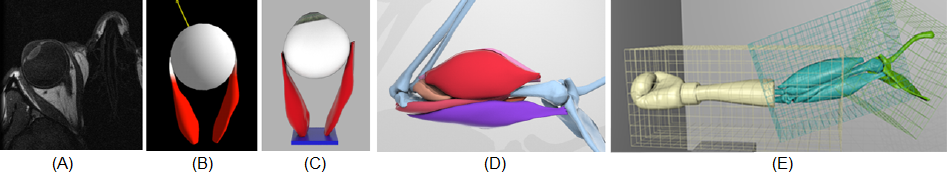
\includegraphics[scale=0.6]{activeVolumetricMuscles.png}
	\caption[Marco de trabajo para simular músculos volumétricos con sólidos Eulerianos-Lagrangianos.]{ El marco de trabajo inicia con la obtención de datos de MRI de la forma activa de músculos (A). Se hace una reconstrucción de la forma de los músculos (B), para posteriormente hacer una simulación del ojo usando el método propuesto (C). Se modelan seis músculos del brazo que están en contacto. La preservación de volumen produce un abultamiento realista (D). Se hace una simulación dinámica de un brazo con tejidos suaves, un guante, y contacto con el ambiente (E).
	Adaptado de \citep{fan2014active}.}
		\label{fig:activeVolumetricMuscles}
\end{figure}

\subsection{Enfoques basados en datos}

En lugar de desarrollar métodos que se enfocan en el modelado de los componentes y procesos físicos de los humanos, se han desarrollado métodos basados en datos que se abstienen de modelar mecanismos anatómicos y se enfocan directamente en la forma de la piel, deformada por el músculo subyacente, de un humano que hace ciertos movimientos o poses. Los datos se capturan en la superficie utilizando sistemas de MOCAP o usando distintos tipos de sensores y dispositivos de medición. Con esos datos, varias técnicas se usan para generar una nueva superficie para simular la piel, dada una pose del esqueleto. Aunque estos enfoques son relativamente nuevos, varios trabajos han mostrado la ventaja que proveen.

Min et al. \citep{min2000anatomically} se basa en que la forma de la piel en un humano es determinada por el esqueleto subyacente y los músculos, y usa un modelo anatómico basado en distintas capas: esqueleto, músculos, y piel. Al mover el esqueleto se deforma la isosuperficie del músculo, preservando el volumen del mismo, que a su vez deforma la capa de la piel. En este trabajo se modeló la parte superior del cuerpo, y la animación resultante muestra el doblado y estiramiento de un brazo. Otro enfoque de animación de brazo es el de Sloan et al. \citep{sloan2001shape}. En éste se utilizaron varias formas de brazo de ejemplo, así como un esquema de interpolación en base a funciones lineales y radiales para crear un rango continuo de poses.

Ma et al. \citep{ma2004realistic} aprovecha el hecho de que empezaron a existir más fuentes de datos con poses de humanos. Utilizando la técnica de escaneo de rango, donde una persona posa por un corto tiempo mientras un escaner crea miles de puntos de datos sobre el sujeto con una densidad de unos milímetros, son capaces de crear un modelo de animación del cuerpo humano. El modelo resultante permite generar animaciones en tiempo real, al manipular el esqueleto mientras se mantiene el nivel de detalle de la superficie del cuerpo humano. Allen et al. \citep{allen2002articulated} crearon un modelo de alta calidad de la parte superior del cuerpo, que es capaz de generar varias poses, basándose en un escaneo de rango. En \citep{allen2003space} se extiende el trabajo previo para incluir los datos de la amplia base de datos de escaneo de rango de cuerpo completo, CAESAR (Civilian American and European Surface Anthropometry Resource project). Morphing (cambio de una imagen u objeto a otro por medio de pasos graduales) por interpolación entre dos escaneos, o el ajuste de un modelo a datos escasos de marcadores de MOCAP, son dos resultados importantes de ésta técnica. También se permitió la transferencia de texturas, datos de superficie, o animaciones entre dos modelos, con el fin de corregir problemas de escaneo, alterar la apariencia, o para animar una gama amplia de personajes. De igual forma, se podían definir varios parámetros extra de una persona, como su altura, o su peso, con el fin de que se consideraran para ser preservadas al momento de modificar una parte de un personaje. Un ejemplo de los personajes que se pueden crear se puede ver en la \fref{fig:dataDrivenModel}.

\begin{figure}
	\centering
		\includegraphics[scale=0.6]{dataDrivenModel.png}
	\caption[Simulación de cuerpos humanoides basada en datos.]{Simulación de cuerpos humanoides basada en datos. Adaptado de \citep{allen2003space}.}
		\label{fig:dataDrivenModel}
\end{figure}

Seo y Thalmann \citep{seo2003automatic} presentan un sistema similar basado en plantillas, con parámetros adicionales para generar nuevas formas humanas que fueran animables al momento. Sand et al. \citep{sand2003continuous} proponen una técnica alternativa, en la que se utilizan siluetas de un video en lugar de datos de escaneo de rango para generar una forma humana que sea animable. Anguelov et al. \citep{anguelov2005scape} extienden ese trabajo, al enfocarse en representar la deformación muscular que se genera como resultado de el movimiento del cuerpo, con el fin de realizar una animación y terminación de la forma de personas (Shape Completion and Animation of People, SCAPE) al usar modelos separados para la deformación de la pose del cuerpo, y para la variación de la forma del cuerpo. Una limitación de éste sistema es que se usa el mismo modelo de deformación muscular para todas las personas generadas, por lo que una persona que sea más muscular puede que no muestre tanta deformación muscular como debería.

\begin{figure}
	\centering
		\includegraphics[scale=0.45]{dataDrivenMoCap.png}
	\caption[Simulación de cuerpos humanoides basada en datos de MOCAP.]{Simulación de cuerpos humanoides basada en datos de MOCAP. Adaptado de \citep{park2008data}.}
		\label{fig:dataDrivenMoCap}
\end{figure}

Park y Hodgins \citep{park2006capturing, park2008data} refinan aún más la deformación de músculos y piel basadas en datos de MOCAP. Ellos modelan deformaciones estáticas como una función de la pose del esqueleto, y las deformaciones dinámicas como una función de la aceleración de cada parte del cuerpo. Para esto, se capturaron movimientos, tanto lentos como rápidos, de un actor usando 350 marcadores en su cuerpo. Los dos tipos de deformación se modelaron y se pudieron generar nuevas animaciones a partir de entre 40 y 50 marcadores, en posteriores sesiones de MOCAP. Aunque este enfoque tiene las limitaciones de que es basado en que un esqueleto genera el movimiento, y que no expresa un movimiento de los músculos sin que existan cambios en los ángulos de las uniones del cuerpo, se producen animaciones de alta calidad. Un ejemplo de estos resultados se puede ver en la \fref{fig:dataDrivenMoCap}.

\section{Control y simulación}

Mientras que en la sección anterior se enfocó en examinar varios trabajos relacionados con la deformación de los músculos esqueléticos, en ésta sección se revisarán los trabajos que se enfocan en el control de los músculos, con el fin de generar movimientos humanos más realistas. 

En general, el sistema musculo-esquelético es modelado como una combinación de tres modelos: dinámicas de activación, dinámicas de contracción, y dinámicas del esqueleto. Las dinámicas de activación describen las relaciones dinámicas entre la excitación neural y la activación de los músculos. Esto es usualmente modelado utilizando ecuaciones diferenciales ordinarias de primer orden (Ordinary Differential Equations, ODEs), de la siguiente forma:

\begin{equation}
	\frac{\mathrm da_j}{\mathrm dt} = (u_j - a_j) \bigg(\frac{u_j}{\tau_{act,j}} + \frac{1 - u_j}{\tau_{deact,j}} \bigg)
\end{equation}

donde $u_j$, $a_j$, $\tau_{act,j}$, y $\tau_{deact,j}$ son la excitación neural, la activación muscular, el tiempo constante de activación, y el tiempo constante de deactivación de un músculo $j$, respectivamente. Las dinámicas de contracción relacionan la activación con las fuerzas musculares resultantes, al tomar en consideración las características físicas de los músculos, como es el arreglo de las fibras musculares y las propiedades pasivas de los tejidos. Normalmente, el modelo de Hill es comúnmente usado para modelar las dinámicas de contracción. Las dinámicas del esqueleto hacen referencia a la relación entre las fuerzas musculares, restricciones externas, y movimientos esqueléticos resultantes:

\begin{equation}
\label{eq:skeletonDynamics}
	M(q)\ddot{q}+c(q,\dot{q})+g(q) - S(q)f_{ext} = R(q)f_{mt}
\end{equation}

donde $q$, $\dot{q}$, $\ddot{q}$ son vectores de las coordenadas generalizadas de las uniones del cuerpo, velocidad, y aceleración, respectivamente. $M(q)$ es una matriz generalizada de inercia, $c(q,\dot{q})$ es el vector generalizado de Coriolis y de fuerzas centrifugales, y $g(q)$ es el vector de fuerzas gravitacionales generalizadas. $S(q)$ y $R(q)$ denotan las matrices de transformación geométrica de las fuerzas externas generalizadas $f_{ext}$ y fuerzas musculotendinosas $f_{mt}$ sobre las fuerzas de las uniones, respectivamente. Al generar el movimiento del esqueleto utilizando la Ecuación \ref{eq:skeletonDynamics}, las fuerzas de los músculos se pueden calcular utilizando perfiles especificados manualmente (por ejemplo, curvas diseñadas \citep{chen1992pump}, sinusoidales \citep{tu1994artificial, zordan2004breathe}, y control basado en key-frame \citep{teran2003finite}) o valores de activación muscular precedidos computacionalmente (por ejemplo, Tsang et al. \citep{tsang2005helping}, Lee y Terzopoulos \citep{lee2006heads}, Sueda et al. \citep{sueda2008musculotendon}). Mientras más aumente la complejidad de los movimientos deseados, o se necesitan representaciones más realistas en una animación, el uso de éstos modelos se vuelve una gran ventaja ya que son consistentes, precisos, y confiables.

En biomecánica, el cómputo de las funciones musculares ha sido estudiado mediante varios experimentos, y se han generado varios modelos que se han validado contra datos experimentales. Sin embargo, la determinación de funciones que modelen el comportamiento de los músculos es un reto debido a la gran cantidad de redundancia de el sistema muscular: el número de músculos que contribuyen a un movimiento es mayor que los grados de libertad relacionados con el movimiento del esqueleto, por lo que se puede generar un problema de indeterminación. Este problema se resuelve comúnmente al utilizar enfoques de optimización, que son clasificados generalmente en optimización estática y dinámica. Usualmente, se definen como optimizaciones finitas, restringidas, y no lineales, y son comúnmente resueltas utilizando métodos de programación secuencial cuadráticos \citep{nocedal2006numerical}.

\subsection{Optimización estática}

La optimización estática, también conocida como dinámica inversa, toma medidas no invasivas de los movimientos del cuerpo, como su posición, velocidad, aceleración, y cargas externas, como entradas a la Ecuación  \ref{eq:skeletonDynamics} para calcular las fuerzas musculares. Un flujo de datos de optimización estática se puede ver en la \fref{fig:estaticOptimization}. Un movimiento instantáneo del esqueleto en cada instante de tiempo es traducido en ecuaciones algebraicas, donde ciertos criterios deseados son especificados (por ejemplo, $0 \leq F_{mt}\leq F_{mt}^{max}$), o en funciones objetivo. Como una función objetivo, la minimización de la fuerza muscular o la amplitud de activación son usualmente usadas:

\begin{equation}
	J = \sum_{i=i}^n \bigg( \frac{F_{mt,i}}{PCSA_i} \bigg)^2
\end{equation}

donde $F_{mt,i}$ es la fuerza aplicada por el músculo $i$ en un instante de tiempo $t$, $PCSA_i$ es el área de la sección transversal del músculo $i$, y $n$ es el número de músculos. En optimización estática, como no hay dependencias dinámicas entre las fuerzas musculares en diferentes instantes de tiempo, no se requiere una integración de tiempo, lo que hace que el problema sea computacionalmente más sencillo. Sin embargo, es difícil integrar la fisiología del músculo (por ejemplo, dinámicas de excitación y activación) así como el objetivo de la tarea motora (por ejemplo, máxima altura de salto). Además, su validez es dependiente de la precisión de las medidas experimentales de movimientos.

\begin{figure}
	\centering
		\includegraphics[scale=0.7]{estaticOptimization.png}
	\caption[Flujo de datos para optimización estática.]{Flujo de datos para optimización estática. Los movimientos del cuerpo son prescritos como entradas, y se determinan las fuerzas musculares como salida. Adaptado de \citep{kutz2004standard}.}
		\label{fig:estaticOptimization}
\end{figure}

Komura et al. \citep{komura1997muscle, komura2000creating} calcularon la activación de los músculos en base a posturas humanas de las extremidades inferiores obtenidas utilizando key-frames, y utilizaron una función objetivo que minimizaba la fuerza muscular y la amplitud de la activación. En \citep{komura2000creating} su modelo fue extendido para considerar características fisiológicas, como la fatiga y lesiones musculares. Tsang et al. \citep{tsang2005helping} presentaron un modelo musculo-tendinoso de una mano humana y de un antebrazo. Utilizando datos de MOCAP o de animación por key-frame, se determina un conjunto de activaciones musculares optimas utilizando optimización estática, y posteriormente se usa como entrada para simular un modelo donde la mano y el antebrazo consiguen realizar una pose o movimiento deseado. 

Lee y Terzopoulos \citep{lee2006heads} desarrollaron un modelo biomecánico del cuello y la cabeza utilizando una estructura jerárquica para generar las simulaciones (ver \fref{fig:headsUp}). Su sistema es controlado por dos subsistemas: un controlador voluntario de alto nivel, y un controlador de reflejos de bajo nivel. El controlador voluntario genera señales neurales anticipadas relacionadas con las poses deseadas, el tono muscular, y una retroalimentación basada en un monitoreo de el movimiento en curso. Cuando el controlador de reflejos recibe esas señales, éste determina como se activan los músculos, y modula los niveles de tensión de los músculos en relación a su estado en curso. Se usa una red neuronal artificial para modelar el controlador voluntario. Éste se entrena fuera de línea utilizando funciones de señales precalculadas de una pose objetivo. Finalmente, para modelar los actuadores de fuerza de cada músculo, se empleó el modelo de músculos de Hill, definiendo cada unidad musculo-tendinosa como un segmento de línea uniaxial sobre el cual se aplica el modelo. 

\begin{figure}
	\centering
		\includegraphics[scale=0.45]{headsUp.png}
	\caption[Simulación neuromuscular de cabeza y cuello.]{Simulación neuromuscular de cabeza y cuello. El sistema biomecánico se compone de esqueleto, músculos, sistema de control neural, y una cara con expresiones. Adaptado de \citep{lee2006heads}.}
		\label{fig:headsUp}
\end{figure}

El trabajo previo fue extendido para simular la parte superior del cuerpo humano, al integrar el torso, y los brazos \citep{lee2009comprehensive}. Además del modelo de dinámica de músculos y esqueletos ya descrito, se incorporó un sistema basado en física para simular el tejido suave del cuerpo, con el fin de representar deformaciones realistas de la carne y la piel durante el movimiento del cuerpo. Su modelo de cuerpo está compuesto de 68 huesos, con 147 grados de libertad, así como de 814 músculos (tanto superficiales, como intermedios, y profundos), cada uno modelado como un segmento de línea con un actuador de fuerza uniaxial de Hill, y cada uno de ellos ejerce una fuerza sobre los huesos relacionados. El modelo completo de la parte superior del cuerpo se puede ver en la \fref{fig:muscleTorso}.

\begin{figure}
	\centering
		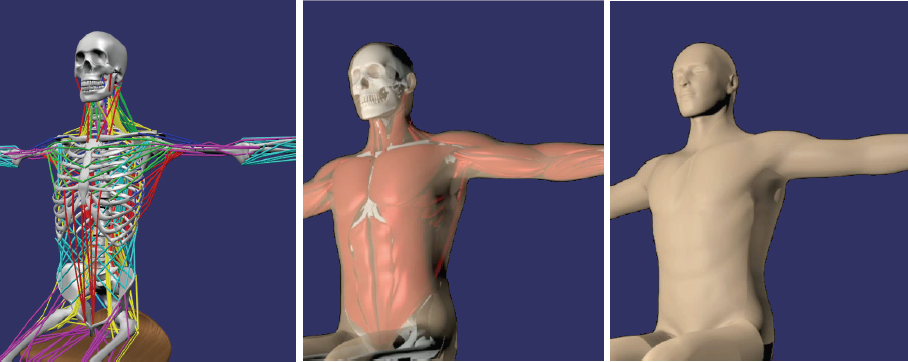
\includegraphics[scale=0.55]{muscleTorso.png}
	\caption[Simulación de la parte superior del cuerpo.]{Modelado exhaustivo de los tejidos relevantes para ejercer control sobre el cuerpo. Se presenta un esqueleto que se mueve con actuadores musculares modelados con un segmento de línea uniaxial de Hill (izquierda). El movimiento generado deforma el tejido suave (centro) y la piel (derecha). Adaptado de \citep{lee2009comprehensive}.}
		\label{fig:muscleTorso}
\end{figure}

Sueda et al. \citep{sueda2008musculotendon} presentan una simulación del sistema musculo-tendinoso de una mano, donde el comportamiento de los músculos y los tendones está dirigido por una dinámica de curvas spline. Esa dinámica se formuló al unir la contracción muscular y las restricciones de fuerzas que se aplican a músculos y tendones. 

\subsection{Optimización dinámica}

La optimización dinámica, también conocida como dinámica directa, es generalmente formulada al combinar la fuerza total generada por la unidad musculotendinosa, las dinámicas de activación, y las dinámicas del esqueleto. Se toma como entrada la exitación de los músculos, usualmente electromiografías, con el fin de producir un movimiento del cuerpo y después determinar la trayectoria de excitación optima. Un flujo de datos de optimización dinámica se puede ver en la \fref{fig:dynamicOptimization}. A diferencia de la optimización estática, que solo toma en cuenta un instante de tiempo, la optimización dinámica considera la duración completa del movimiento, necesitando una integración de tiempo de la ecuación \ref{eq:skeletonDynamics}. Por esto, la optimización dinámica es mucho más computacionalmente demandante que la estática. Sin embargo, a diferencia de la optimización estática, se pueden incluid propiedades fisiológicas, o que dependen del tiempo, como saltos intentando alcanzar la mayor altura posible \citep{pandy1990optimal}, saltos verticales en tres dimensiones \citep{anderson1999dynamic}, o caminado \citep{anderson2001dynamic}. En el caso de Anderson y Pandy \citep{anderson2001dynamic, anderson2001static} se empleó la minimización de gasto de energía metabólica por unidad de distancia durante el caminado normal humano. 

En \citep{anderson2001static}, Anderson y Pandy demostraron que la optimización estática y dinámica generan virtualmente los mismos resultados en cuanto a la predicción de las fuerzas musculares y las fuerzas de contracción durante un caminado normal humano. Ellos argumentan que esa similaridad se da ya que el minimizar la fatiga muscular en cada instante de tiempo es casi lo mismo que minimizar la energía metabólica gastada por unidad de distancia recorrida para completar un ciclo de caminado. Además, comentan que ciertas propiedades fisiológicas, como las de fuerza, longitud, y velocidad de los músculos, así como las dinámicas de activación, tienen poca influencia en la optimización estática.

\begin{figure}
	\centering
		\includegraphics[scale=0.7]{dynamicOptimization.png}
	\caption[Flujo de datos para optimización dinámica.]{Flujo de datos para optimización dinámica. Una señal de excitación de los músculos se toma como entrada, y el movimiento muscular resultante es usado para determinar una excitación optima. Adaptado de \citep{kutz2004standard}.}
		\label{fig:dynamicOptimization}
\end{figure}

\section{Simulación basada en fibras}

Como se puede ver en secciones anteriores, los modelos musculares presentados en la literatura usualmente utilizan modelos fenomenológicos, y se enfocan en los músculos como un todo, sin prestar atención a las estructuras internas. Normalmente, éstos representan la anatomía real de los músculos con geometrías simplificadas con el fin de minimizar los costos computacionales o para poder aplicar los modelos fenomenológicos a sus simulaciones. Simulaciones basadas en mecánicas de sólidos, como los basados en FEM o FVM, tienen que utilizar técnicas variadas para detectar colisiones, y simular el efecto de contacto entre los músculos. Sin embargo, esas técnicas son caras computacionalmente, y no funcionan muy bien con cuerpos deformables. Además, las primitivas básicas de esos modelos, como tetraedros o hexaedros, no se deforman de la misma manera que las fibras musculares \citep{pai2011dynamics}. 

Además, la mayoría de los trabajos presentados utilizan modelos fenomenológicos para simular las fuerzas que producen los músculos; en específico, se usa el modelo de músculos de Hill. Los modelos musculares basados en el trabajo de Hill tienen ciertas limitaciones. Una de las principales es que las fuerzas producidas por estos modelos se aplican a lo largo de una línea de acción representada como un segmento de línea en una dimensión que se une a los huesos del cuerpo sobre los que actúa. Sin embargo, la forma en tres dimensiones de los músculos y las fuerzas intermusculares a menudo se pasan por alto, o se simplifican. Otro problema con éste tipo de modelos es el que encontraron Epstein et al \citep{epstein2006should}. En su trabajo demuestran que los modelos donde se simplifican las fibras musculares, la aponeurosis, y los tendones, tienden a generar fuerzas de transmisión erróneas, y que es necesario considerar todas las relaciones entre las fibras musculares, los tejidos conectivos, la aponeurosis, y los tendones. De igual manera, Herzog \citep{herzog2004history} encontró que en los modelos de músculos de Hill se pueden generar errores en la producción de fuerza de hasta 50\%, en comparación con fuerzas de referencia isométricas de músculos humanos, aún en escenarios controlados.

Los siguientes trabajos se enfocan en hacer simulaciones de los músculos considerando las distintas estructuras internas, enfocándose principalmente a las fibras musculares. Además, emplean distintos modelos biofísicos para simular la contracción de las fibras y la generación de fuerza de los músculos.

Ng-Thow-Hing et al. \citep{ng1998shape} definen sólidos B-spline (extensión de las curvas y las superficies B-spline a un dominio de volumen) para crear modelos deformables con forma de músculos. Para obtener la forma de los músculos se utilizaron datos de músculos a través de imágenes de The Visible Human Project \citep{visibleHumanProject}. Aunque esas imágenes dan una indicación de el perímetro del músculo, no proveen información del arreglo interno de las fibras musculares; para obtener las coordenadas de los grupos de fibras musculares se hizo una triangulación óptica de imágenes de tres cámaras de especímenes diseccionados en serie del músculo sóleo de la pierna. Utilizando la información de el arreglo de las fibras, generaron un método para ajustar un sólido B-spline a las fibras, y así poder tener un sólido basado en fibras que se aproxime al músculo. Para poder deformar el músculo generado, se aplicó una red viscoelástica a los puntos de control del sólido. 

En \citep{ng1999physically} el trabajo previo se extiende para incluir: colisiones entre músculos utilizando un método que encuentra los puntos más cercanos a un sólido; agregar puntos de masa a los puntos de control, para permitir reacciones físicas del músculo, y poder aplicar fuerzas musculares a los puntos de masa; usar ecuaciones Lagrangianas para tener preservación de volúmen; y finalmente utilizar las fibras como generadores de fuerza sobre huesos y generar movimiento. En la \fref{fig:bsplineSolidFibers} se puede ver el arreglo de fibras y el sólido B-spline resultante. En \citep{ng2001muscle}, se continúa el trabajo previo al incluir la aponeurosis de los músculos, y se incluye un modelo de fuerzas para cada fibra. La aponeurosis se modela como una hoja elástica que restringe la deformación del músculo sóleo a lo largo de las superficies donde está unido. Cada fibra tiene un modelo de Hill que le permite contraerse y genera una distribución no uniforme de las fuerzas contráctiles dentro del mismo músculo.

\begin{figure}
	\centering
		\includegraphics[scale=0.7]{bsplineSolidFibers.png}
	\caption[Simulación de músculos con sólidos B-spline.]{En la parte izquierda se muestran las fibras que están dentro del sólido B-spline. En la parte derecha se muestra como los músculos están unidos a los huesos y su deformación al generar un movimiento de rotación. Adaptado de \citep{ng1999physically}.}
		\label{fig:bsplineSolidFibers}
\end{figure}

Blemker y Delp \citep{blemker2005three} crearon mallas de FEM en tres dimensiones de la forma de los músculos en base a MRI, y desarrollaron un método para prescribir la geometría de las fibras musculares dentro de la malla, dependiendo de la arquitectura de cada músculo. Su método se basa en plantillas en forma de cubo de la geometría de las fibras musculares, que posteriormente se ajustan para crear la geometría de las fibras dentro del músculo. Para lograr ésto, la plantilla cúbica se divide en varias secciones, que posteriormente se proyectan a secciones similares de la malla objetivo. La base de cada plantilla de geometría de fibras es una interpolación entre múltiples curvas B-spline, para simular las diferentes arquitecturas musculares. En la \fref{fig:templateProjection} se puede ver el proceso mencionado. Una desventaja de éste método es que es muy impráctico para representar músculos en tres dimensiones, debido a que el costo computacional de simular las mallas finales es alto. Esto hace que no sea viable integrarlas con simulaciones que ya son caras, como controlar la dinámica de movimiento de los músculos.

\begin{figure}
	\centering
		\includegraphics[scale=0.7]{templateProjection.png}
	\caption[Generación de geometría de fibras a través de plantillas.]{Creación de la geometría de fibras musculares para una malla de músculo generada a través de MRI. Secciones de una plantilla (A) se proyectan sobre una malla objetivo (B) para generar una malla con forma de músculo con fibras musculares (C). Adaptado de \citep{blemker2005three}.}
		\label{fig:templateProjection}
\end{figure}

Kohout et al. \citep{kohout2012muscle} presentan un método para representar los músculos mediante grupos realistas de fibras musculares que se generan automáticamente en un volumen definido por una malla de un músculo. Su implementación puede descomponer el volumen de un músculo en fibras musculares al ir ajustando una plantilla de fibras al volumen del músculo. Sin embargo, su modelo no tiene consideraciones biomecánicas, y puede producir caminos de fibras poco realistas, y que no estén cerca de sus puntos reales de unión al hueso.

%A diferencia de los trabajos previos, donde se usan plantillas de fibras para modelar la geometría de las fibras musculares, Choi y Blemker \citep{choi2013skeletal} proponen el uso de vectores de campo Laplacianos libres de rotaciones y divergencias para modelar los fascículos de los músculos. Éste trabajo se basa en que la contracción y fuerza musculares son generados por las fibras musculares agrupadas dentro de fascículos, y que no habían representaciones adecuadas del arreglo de los .
%
%--Skeletal muscles are characterized by a large diversity in anatomical architecture and function. Muscle force and contraction are generated by contractile fiber cells grouped in fascicle bundles, which transmit the mechanical action between origin and insertion attachments of the muscle. Therefore, an adequate representation of fascicle arrangements in computational models of skeletal muscles is important, especially when investigating three-dimensional muscle deformations in finite element models. we present an alternative approach based on the
%hypothesis of a rotation and divergence free (Laplacian) vector field behavior which reflects observed physical
%characteristics of fascicle trajectories. To obtain this representation, the Laplace equation was solved in anatomical
%reconstructions of skeletal muscle shapes based on medical images using a uniform flux boundary condition on the attachment areas. Fascicle tracts were generated through a robust flux based tracing algorithm.
%--The method is based on the observation that fascicle trajectories have the following properties: (i) they are co-axially aligned and hence do not cross ach other, (ii) they do not branch, (iii) they will not reverse their irections abruptly, and (iv) they must connect between the tendon or bone attachments to convey mechanical action, which means that they only originate or terminate in areas of origin (proximal) and insertion (distal). Based on these observations, we hypothesize that fascicle arrangements in skeletal muscles can be mathematically represented by a rotation and divergence free Laplacian vector field.


Tang et al. \citep{tang20093d} presentan un modelo de FEM en tres dimensiones para simular los comportamientos mecánicos de los músculos durante su alargamiento o acortamiento. El músculo completo se modela como un material hiperelástico con fibras musculares activas. Su modelo considera que las fibras musculares van a unir dos puntos centrales de hexaedros que forman la malla final del músculo. Las propiedades mecánicas de las fibras musculares se describen en base al modelo de músculos de Hill. Sin embargo, su modelo se restringe a aplicaciones donde el músculo se modele como hexaedros ordenados, y no se puede aplicar a modelos con geometrías más complejas. 

R{\"o}hrle \citep{rohrle2010simulating} desarrolló un modelo electromecánico de los músculos esqueletales. El modelo acopla las propiedades electro-fisiológicas a nivel celular (la unidad contráctil del músculo) con los principios biomecánicos a nivel del órgano (el músculo completo), enfocándose en la generación de fuerza del músculo. Para modelar la actividad eléctrica de las fibras musculares, sin describir las propiedades electro-fisiológicas de una sola célula, es resolviendo las ecuaciones bidominio \citep{vigmond2002computational, rohrle2010simulating, rohrle2012physiologically}. Esas ecuaciones proveen un enfoque de modelado continuo, donde los espacios extracelulares e intracelulares son modelados como si ocuparan el mismo espacio. Finalmente, se generan ecuaciones de fuerza para manejar la contracción muscular, considerando como entrada al sistema una corriente eléctrica, que inerva las fibras. Las fibras musculares se modelan como objetos de una dimensión, que son discretizadas utilizando elementos finitos lineales de una dimensión de Lagrange. Esas fibras se alinean en un espacio de tres dimensiones a lo largo de la dirección real de las fibras de un músculo (esos datos se obtuvieron de \citep{visibleHumanProject}). También se incluye un nivel de detalle para la graficación de las fibras, donde se puede determinar si una cadena de una dimensión representa un fascículo, una fibra, o un grupo de fibras.

\begin{figure}
	\centering
		\includegraphics[scale=0.5]{femMotorUnits.png}
	\caption[Simulación de fibras musculares y las unidades motoras relacionadas.]{Se muestra el músculo tibial anterior, en color azul (A). Se muestra una unidad motora, y las fibras musculares relacionadas a esa unidad (B). Se muestran las fibras musculares relacionadas con 5 (C) y con 10 (D) unidades motoras. Adaptado de \citep{rohrle2012physiologically}.}
		\label{fig:femMotorUnits}
\end{figure}

R{\"o}hrle et al. \citep{rohrle2012physiologically} extienden el trabajo previo al presentar un modelo fisiológico de los músculos esqueletales que es capaz de representar descripciones geométricas de las fibras musculares y su agrupamiento. En conjunto con un modelo de activación de neuronas motoras en los músculos, el comportamiento electro-fisiológico de las fibras musculares dentro de una unidad motora se calcula y se aplica para obtener las fuerzas musculares que generan movimientos. En éste caso, se considera que todas las fibras se inervan en su punto medio, por lo que es suficiente modelar la activación de una fibra muscular por unidad motora, y usar su salida para todas las otras fibras asociadas. Las fibras están dentro de una malla de elemento finito, anatómicamente realista generado a partir de imágenes de \citep{visibleHumanProject}, del músculo tibial anterior. El modelo presentado también es capaz de simular la fatiga generada en los músculos. En la \fref{fig:femMotorUnits} se puede ver el arreglo de fibras musculares para diferentes unidades motoras.

\begin{figure}
	\centering
		\includegraphics[scale=0.7]{strandsShoulderHand.png}
	\caption[Simulación de hombro y mano utilizano strands.]{En la izquierda se muestra una simulación del hombro modelando los músculos con strands. En la derecha se muestra una simulación de los movimientos de una mano utilizando strands. Adaptado de \citep{pai2011dynamics}.}
		\label{fig:strandsShoulderHand}
\end{figure}

Pai et al. \citep{pai2011dynamics} hacen un análisis de las deficiencias de las simulaciones de músculos previas, y propone un modelo muscular basado en fibras para considerar propiedades biofísicas que no habían sido consideradas. Mencionan que en simulaciones anteriores, no se considera correctamente la masa muscular. Una forma conveniente de considerarla era unirla con la masa de los huesos y la de el tejido suave a lo largo de un segmento del cuerpo. Sin embargo, cuando el  músculo se estira o se acorta, la masa muscular también se mueve en la dirección del estiramiento o la contracción, y va a contribuir a la inercia del sistema. Otro problema que encuentran en las simulaciones anteriores es que los sistemas musculo-esqueléticos no pueden tratar correctamente con el contacto y con restricciones de enrutamiento. Finalmente mencionan que las simulaciones basadas en FEM o FVM, no son ideales para simulaciones con elementos juntos o apretados, ya que se requiere de detección de colisiones y de algoritmos de resolución, que son caros computacionalmente y no trabajan bien con objetos deformables. Por esas limitaciones, proponen un simulador de strands que sea capaz de simular tejidos parecidos a fibras, suaves, delgados, con propiedades biofísicas, y capaces de tener restricciones complejas de enrutamiento (como las que tienen los tendones, músculos, y ligamentos). Usando la terminología de Pai \citep{pai2002strands}, se usa el término \textit{strand} para indicar que las fibras no solamente son curvas en un espacio, si no que tienen  masa, elasticidad, y otras propiedades físicas que influencian su dinámica. En la figura \fref{fig:strandsShoulderHand} se pueden ver dos simulaciones resultantes de el simulador propuesto.

% Dejar al final la aponeuroris: Computational representation of the aponeuroses as NURBS